% ============================================================
%  NLP501 – AI in Production: From Models to Systems
%  Final Project Report – Sentiment Analysis Service
%  Team: Dương Hồng Quân · Phạm Đức Long · Đỗ Quốc Trung
% ============================================================
\documentclass[12pt, a4paper]{article}

% ---- Encoding & Language (pdfLaTeX) ----
\usepackage[T1]{fontenc}
\usepackage[utf8]{inputenc}
\usepackage[english]{babel}
\usepackage{lmodern}

% ---- Global overflow prevention ----
\sloppy
\setlength{\emergencystretch}{3em}
\hfuzz=5pt
\usepackage[hyphens]{url}
\usepackage{xurl}

% ---- Layout ----
\usepackage[top=2.5cm, bottom=2.5cm, left=2.8cm, right=2.8cm, headheight=15pt]{geometry}
\usepackage{setspace}
\onehalfspacing

% ---- Typography ----
\usepackage{microtype}
\usepackage{parskip}

% ---- Mathematics ----
\usepackage{amsmath, amssymb}

% ---- Graphics & Colour ----
\usepackage{graphicx}
\usepackage[dvipsnames, svgnames, x11names]{xcolor}
\usepackage{tikz}
\usetikzlibrary{shapes.geometric, arrows.meta, positioning, fit, backgrounds, calc, shadows}

% ---- Tables ----
\usepackage{booktabs}
\usepackage{tabularx}
\usepackage{multirow}
\usepackage{array}
% New column type: P{width} = centered fixed-width; R = right-aligned X
\newcolumntype{P}[1]{>{\centering\arraybackslash}p{#1}}
\newcolumntype{R}{>{\raggedleft\arraybackslash}X}
% All tables get small font by default
\AtBeginEnvironment{tabularx}{\small}
\AtBeginEnvironment{tabular}{\small}

% ---- Code listings ----
\usepackage{listings}
\definecolor{codegreen}{rgb}{0.2,0.6,0.2}
\definecolor{codegray}{rgb}{0.45,0.45,0.45}
\definecolor{codepurple}{rgb}{0.5,0,0.65}
\definecolor{backcolour}{RGB}{248,248,248}
\lstdefinestyle{pythonstyle}{
    backgroundcolor=\color{backcolour},
    commentstyle=\color{codegray}\itshape,
    keywordstyle=\color{NavyBlue}\bfseries,
    numberstyle=\tiny\color{codegray},
    stringstyle=\color{codegreen},
    basicstyle=\ttfamily\footnotesize,
    breakatwhitespace=false,
    breaklines=true,
    breakindent=0pt,
    captionpos=b,
    keepspaces=true,
    numbers=left,
    numbersep=6pt,
    showspaces=false,
    showstringspaces=false,
    tabsize=4,
    frame=single,
    rulecolor=\color{gray!40},
    xleftmargin=1.5em,
    columns=fullflexible,
}
\lstdefinestyle{yamlstyle}{
    backgroundcolor=\color{backcolour},
    commentstyle=\color{codegray}\itshape,
    keywordstyle=\color{DarkOrchid},
    basicstyle=\ttfamily\footnotesize,
    breaklines=true,
    captionpos=b,
    frame=single,
    rulecolor=\color{gray!40},
    xleftmargin=0.5em,
}
\lstset{style=pythonstyle}

% ---- Hyperlinks ----
\usepackage[hidelinks, colorlinks=true, linkcolor=NavyBlue,
            urlcolor=NavyBlue, citecolor=NavyBlue]{hyperref}
\usepackage[strings]{underscore}

% ---- Header & Footer ----
\usepackage{fancyhdr}
\pagestyle{fancy}
\fancyhf{}
\rhead{\small NLP501 -- Sentiment Analysis Service}
\lhead{\small Final Project Report}
\rfoot{\thepage}
\renewcommand{\headrulewidth}{0.4pt}

% ---- Section styling ----
\usepackage{titlesec}
\titleformat{\section}[block]{\Large\bfseries\color{NavyBlue}}{{\thesection}}{1em}{}[\vspace{0.1em}\titlerule]
\titleformat{\subsection}[block]{\large\bfseries\color{MidnightBlue}}{{\thesubsection}}{1em}{}
\titleformat{\subsubsection}[block]{\normalsize\bfseries}{{\thesubsubsection}}{1em}{}

% ---- Misc ----
\usepackage{enumitem}
\usepackage{caption}
\usepackage{subcaption}
\usepackage{float}

% ============================================================
%  Begin Document
% ============================================================
\begin{document}

% ============================================================
%  TITLE PAGE
% ============================================================
\begin{titlepage}
\thispagestyle{empty}
\centering

{\color{NavyBlue}\rule{\linewidth}{3pt}}\\[0.3em]
{\color{SteelBlue}\rule{\linewidth}{1pt}}\\[1.2cm]

{\Large\bfseries\color{NavyBlue} FPT UNIVERSITY}\\[0.3em]
{\large\bfseries\color{MidnightBlue} FSB Institute of Management and Technology}\\[0.2em]
{\small\color{gray} (Vien Quan tri \& Cong nghe FSB, Truong Dai hoc FPT)}\\[1.2cm]

{\Large\bfseries\color{NavyBlue} FINAL PROJECT REPORT}\\[0.6em]
{\color{SteelBlue}\rule{0.62\linewidth}{0.8pt}}\\[0.9cm]

{\Huge\bfseries\color{NavyBlue} Natural Language Processing Sentiment Analysis Platform}\\[0.4em]
{\large\itshape\color{MidnightBlue} Sentiment Analysis Service for Multilingual Review Intelligence}\\[1.0cm]

\colorbox{NavyBlue!12}{%
  \begin{minipage}{0.8\textwidth}\centering\vspace{0.35em}
    {\small\bfseries Course:} {\small NLP501 -- AI in Production: From Models to Systems}\\[0.2em]
    {\small\bfseries Topic:} {\small NLP -- Sentiment Analysis Service}\\[0.2em]
    {\small\bfseries Academic Year:} {\small 2025 -- 2026}\\[0.2em]
    {\small\bfseries Dataset family:} {\small SemEval-2014, tweet\_eval\_irony, multilingual\_sentiment}\vspace{0.35em}
  \end{minipage}
}\\[1.1cm]
{\large\bfseries\color{NavyBlue} PROJECT TEAM}\\[0.8em]

\renewcommand{\arraystretch}{1.3}

\begin{tabularx}{0.9\textwidth}{@{}p{4cm}X@{}}
\toprule
\textbf{Role} & \textbf{Name} \\
\midrule
Tech Lead & Le Quang Tuyen \\

Solution Engineer & Duong Hong Quan \\

ML Engineer & Duong Binh An \\

AI Engineer & Do Quoc Trung \\

Backend Engineer & Pham Duc Long \\

UI/UX Engineer & Nguyen Le Hong Nhi \\
\bottomrule
\end{tabularx}

\vspace{0.95cm}
\colorbox{NavyBlue!8}{%
  \begin{minipage}{0.72\textwidth}
    \centering
    \vspace{0.45em}
    \begin{tabular}{@{}>{\bfseries}r@{\hspace{0.9em}}l@{}}
      Instructor: & Le Thanh Hai \\
      Submission: & June 2026 \\
      Academic Year: & 2025 -- 2026 \\
    \end{tabular}
    \vspace{0.45em}
  \end{minipage}
}

\vfill
{\color{SteelBlue}\rule{\linewidth}{1pt}}\\[0.25em]
{\color{NavyBlue}\rule{\linewidth}{3pt}}
\end{titlepage}
\newpage

\begin{abstract}
This project presents a complete natural language processing platform for sentiment analysis, aspect-based sentiment analysis, sarcasm detection, explainability, data versioning, model training, and production deployment. The system was implemented as a full-stack engineering project using a web frontend, a REST backend, container-based deployment, Prometheus/Grafana observability, and MLflow/DVC for reproducible machine-learning workflows.

The core inference service supports multiple execution modes. In baseline mode the platform uses a pretrained transformer for direct sentiment inference; in fine-tuned mode it uses a multilingual transformer with PEFT/LoRA adapters for sentiment and sarcasm tasks; and in ONNX modes it serves exported FP32 or INT8 models through ONNX Runtime. Aspect-based sentiment analysis is implemented through a zero-shot classifier, while token-level explainability is provided by SHAP. Language support is enforced at the backend level through a lightweight local detector that accepts English and Vietnamese.

The project addresses the operational problem of converting unstructured customer feedback into structured, machine-readable sentiment signals that can support review monitoring, customer-service triage, and product analysis. The implementation includes a reproducible data pipeline for dataset ingestion, preprocessing, validation, training preparation, evaluation, and ONNX export; experiment tracking for metrics and artifacts; request and inference monitoring; and automated checks for code quality and test execution.

Evaluation artifacts in the repository show a baseline test-set result of 0.8135 accuracy and 0.7389 macro F1 on 799 SemEval test samples, together with a fine-tuned evaluation artifact reporting 0.7926 overall F1 on a sampled evaluation run. Data-quality validation reports a clean processed dataset of 3,831 samples with zero null-ratio violations and one distribution warning for the missing location aspect category. The repository also contains ONNX benchmark artifacts, fairness reports, SHAP visualization outputs, and deployment configuration for a production-style multi-service stack.

The main contribution of the project is not a single model checkpoint but an end-to-end sentiment analysis system with reproducible engineering controls, model explainability, monitoring, and deployment artifacts. The platform also documents explicit limitations, including the absence of authenticated access control, the mock nature of the batch-status workflow, and the fact that document/audio upload capabilities described in frontend notes are not implemented in the backend.
\end{abstract}

\newpage
\tableofcontents
\newpage

% ============================================================
\section{Chapter 1 Introduction}
% ============================================================

\subsection{Background}
Sentiment analysis is the task of identifying the emotional or evaluative orientation expressed in text. In modern NLP systems it is commonly applied to customer reviews, social posts, survey responses, and support tickets. The repository implements this problem in a restaurant-review domain using transformer-based text classification, aspect-based sentiment analysis, sarcasm detection, and post-hoc explainability.

The practical value of sentiment analysis comes from its ability to transform unstructured feedback into structured evidence. The platform is designed for customer-feedback interpretation, where the same input can be evaluated at the sentence level and at the aspect level. The design combines overall sentiment, ABSA, and SHAP explanations into a single response.

\subsection{Problem Statement}
Manual sentiment inspection does not scale to large feedback streams and introduces inconsistency across reviewers. It is also difficult to use manually generated sentiment labels in downstream systems because the output is not machine-readable, not reproducible, and not directly measurable. The project addresses this by implementing an API-based pipeline that produces deterministic model outputs, machine-readable response schemas, and monitoring signals suitable for production deployment.

\subsection{Project Objectives}
\begin{table}[H]
\centering
\caption{Project objectives by layer}
\begin{tabularx}{\textwidth}{@{} p{3.1cm} X @{}}
\toprule
\textbf{Objective type} & \textbf{Implemented objective} \\
\midrule
Functional objectives & Single prediction, batch CSV prediction, SHAP explanation, health check, and evaluation trigger endpoints. \\
Technical objectives & Typed API contracts, DVC-managed data flow, MLflow experiment tracking, ONNX export, Prometheus metrics, and Docker deployment. \\
AI objectives & Multilingual sentiment inference, sarcasm detection via a second adapter, aspect-based sentiment extraction, and token-level explainability. \\
Deployment objectives & Multi-service container deployment using Docker Compose with frontend, backend, monitoring, and tracking services. \\
\bottomrule
\end{tabularx}
\end{table}

\subsection{Scope}
\begin{table}[H]
\centering
\caption{Scope definition}
\begin{tabularx}{\textwidth}{@{} p{3cm} X @{}}
\toprule
\textbf{In Scope} & \textbf{Out of Scope} \\
\midrule
Single and batch inference, ABSA, SHAP explainability, language detection, DVC data processing, LoRA fine-tuning, ONNX export, metrics, dashboards, alerting, and test automation. & User authentication, rate limiting, online learning, active learning, real-time message queues, document upload, audio upload, and fully asynchronous batch-job orchestration. \\
\bottomrule
\end{tabularx}
\end{table}

\subsection{Contributions}
\begin{itemize}[noitemsep]
  \item Built a backend service in FastAPI with typed request and response schemas.
  \item Implemented a configurable inference engine with baseline, finetuned, and ONNX execution modes.
  \item Added ABSA through zero-shot classification and added sarcasm detection through a dedicated adapter path.
  \item Implemented SHAP-based explanation generation and frontend explanation rendering.
  \item Built a DVC pipeline for raw data extraction, preprocessing, validation, training preparation, evaluation, and export.
  \item Added MLflow logging for evaluation and training runs.
  \item Added Prometheus metrics, alert rules, and Grafana provisioning.
  \item Built an Angular frontend with chat interaction, batch CSV upload, theme switching, and explainability display.
\end{itemize}

% ============================================================
\section{Chapter 2 Literature Review and Theoretical Foundation}
% ============================================================

\subsection{Sentiment Analysis}
Sentiment analysis studies how opinions, preferences, emotions, and evaluations can be inferred from text. In practice, the task has evolved from lexicon-based polarity scoring to supervised neural classification and, more recently, to transformer-based language understanding. The project uses this classical sentiment classification problem as the primary interface for customer-feedback intelligence.

The main challenge in sentiment analysis is that opinion polarity is often context-dependent. Negation, contrastive conjunctions, intensifiers, domain-specific vocabulary, and sarcasm can all alter the surface meaning of a sentence. For that reason, the project does not rely on a single label only; it combines sentence-level sentiment, aspect-level sentiment, sarcasm detection, and explainability to reduce ambiguity in interpretation.

\subsection{Aspect-Based Sentiment Analysis}
Aspect-based sentiment analysis decomposes a review into semantically meaningful targets such as food, service, ambiance, price, or location, and then estimates the polarity associated with each target. This is more useful than a single document-level label when the same review contains mixed opinions. A customer may praise the food while criticizing the service, and a document-level classifier would otherwise collapse that distinction.

The project adopts a pragmatic ABSA design based on zero-shot inference. This choice avoids the need for a separate annotated ABSA corpus for every domain-specific aspect while still enabling structured output. The trade-off is that zero-shot ABSA is more sensitive to prompt phrasing and may be less stable than a domain-trained aspect classifier.

\begin{table}[H]
\centering
\caption{Sentiment analysis research concepts and project usage}
\begin{tabularx}{\textwidth}{@{} p{3.5cm} p{3.2cm} X @{}}
\toprule
\textbf{Concept} & \textbf{Role in theory} & \textbf{Role in this project} \\
\midrule
Document sentiment & Estimates overall polarity of a text. & Forms the primary prediction returned by the platform. \\
Aspect sentiment & Associates polarity with a specific target. & Produces structured feedback for food, service, and related aspects. \\
Sarcasm/irony & Handles polarity reversal and figurative language. & Provides an auxiliary binary signal for difficult samples. \\
Explainability & Makes prediction evidence visible. & Returns SHAP token contributions for user inspection. \\
\bottomrule
\end{tabularx}
\end{table}

\subsection{Transformer Architecture}
Transformer models address sequence modeling through tokenization, embedding, attention, and stacked encoder blocks. Tokenization converts raw text into subword units, which helps the model handle rare words and multilingual text. Embeddings map these tokens into dense vectors, while self-attention computes token-to-token interactions so the model can represent context.

For classification, the project uses a transformer encoder followed by a classification head. The head maps the final hidden representation to class probabilities. This design is well suited to sentiment analysis because it captures both local cues and longer-range dependencies without requiring recurrent computation.

\subsection{Multilingual NLP}
Multilingual NLP extends the same modeling framework across languages. The main challenges are script variation, tokenization differences, vocabulary imbalance, and uneven data availability. The project handles multilingual input by using a multilingual backbone and a lightweight language gate that accepts English and Vietnamese inputs. This design is narrow but deliberate: it avoids overclaiming broad multilingual coverage while still supporting the datasets actually used in the repository.

\subsection{PEFT and LoRA}
Parameter-efficient fine-tuning modifies only a small subset of model parameters, which lowers compute cost and storage requirements. LoRA is the mechanism used in this project: low-rank matrices are injected into selected attention projections, allowing the backbone to remain mostly frozen while task-specific behavior is learned in compact adapter weights.

The primary advantage of LoRA is that it reduces training cost and makes it practical to maintain separate adapters for different tasks, such as sentiment and sarcasm detection. The main trade-off is that task adaptation capacity is constrained by the low-rank approximation, so performance can lag behind a full fine-tune if enough data and compute are available.

\subsection{Explainable AI}
Explainable AI is important in sentiment systems because a prediction is often only useful if users can understand why it was made. SHAP is used in this project because it provides a consistent additive explanation framework grounded in Shapley value theory. Each token receives a contribution score that reflects how much it supports or suppresses the predicted class relative to a baseline.

The explanation interface is intended for human review rather than formal audit. It helps a lecturer, examiner, or evaluator understand whether the model is reacting to sentiment-bearing words, negation, or aspect-specific terms. The repository does not include a dedicated explanation-fidelity benchmark, so the explainability layer is validated qualitatively through visual inspection.

\subsection{MLOps Concepts}
The system reflects several MLOps concepts: DVC is used to make data and pipeline stages reproducible, MLflow is used to track metrics and artifacts, monitoring is used to observe runtime behavior, and containerization is used to preserve execution consistency. These tools provide the operational bridge between model development and deployable software.

\begin{table}[H]
\centering
\caption{Theoretical concepts and engineering implications}
\begin{tabularx}{\textwidth}{@{} p{3.5cm} X @{}}
\toprule
\textbf{Concept} & \textbf{Engineering implication} \\
\midrule
Transformer self-attention & Better handling of context and long-distance dependency. \\
PEFT / LoRA & Lower training cost and easier adapter management. \\
SHAP explainability & User-facing interpretability and token-level evidence. \\
MLOps toolchain & Reproducible datasets, experiments, and deployment artifacts. \\
\bottomrule
\end{tabularx}
\end{table}

% ============================================================
\section{Chapter 3 Requirements Analysis}
% ============================================================

\subsection{Stakeholders}
\begin{table}[H]
\centering
\caption{Stakeholder analysis}
\begin{tabularx}{\textwidth}{@{} p{3.2cm} X @{}}
\toprule
\textbf{Stakeholder} & \textbf{Role in the system} \\
\midrule
Users & Submit text, inspect sentiment, view aspect-level results, and request explanations through the frontend or HTTP API. \\
Administrators & Operate the deployment stack, monitor uptime, and inspect metrics and dashboards. \\
Developers & Extend the backend, frontend, pipeline, tests, and deployment configuration. \\
Researchers & Reproduce experiments, review metrics, and inspect generated artifacts such as fairness reports and SHAP plots. \\
\bottomrule
\end{tabularx}
\end{table}

\subsection{Functional Requirements}
\begin{table}[H]
\centering
\caption{Functional requirement matrix}
\begin{tabularx}{\textwidth}{@{} p{1.5cm} p{1.8cm} p{3.2cm} X @{}}
\toprule
\textbf{ID} & \textbf{Priority} & \textbf{Requirement} & \textbf{Implementation evidence} \\
\midrule
FR-01 & Must & Predict sentiment for a single text input. & The platform returns an overall sentiment label and confidence score for a single submitted message. \\
FR-02 & Must & Return aspect-level sentiment alongside the overall label. & The platform identifies supported aspects and returns per-aspect sentiment for each relevant category. \\
FR-03 & Must & Provide SHAP-based explanations. & The platform exposes token-level explanation values for a submitted prediction. \\
FR-04 & Must & Support CSV batch prediction. & The platform accepts a CSV file, validates the expected text column, and returns row-level inference results. \\
FR-05 & Must & Expose health information. & The platform reports model availability and supported language coverage. \\
FR-06 & Should & Detect language and reject unsupported languages. & The platform detects English and Vietnamese inputs and rejects unsupported languages. \\
FR-07 & Must & Expose Prometheus metrics. & The platform exports operational metrics for scraping. \\
FR-08 & Must & Evaluate the model and log artifacts. & The platform can run evaluation workflows and persist metrics artifacts. \\
FR-09 & Should & Provide a usable browser frontend. & A browser-based interface supports chat-style interaction and batch analysis. \\
FR-10 & Should & Support monitoring and alerting. & The deployment includes scraping and alerting configuration for operational visibility. \\
\bottomrule
\end{tabularx}
\end{table}

\subsection{Non-Functional Requirements}
\begin{table}[H]
\centering
\caption{Non-functional requirements}
\begin{tabularx}{\textwidth}{@{} p{2.6cm} p{3cm} X @{}}
\toprule
\textbf{Category} & \textbf{Requirement} & \textbf{Evidence} \\
\midrule
Performance & Keep inference usable on CPU and support ONNX acceleration. & The system provides a CPU-oriented runtime path and exported ONNX models for lower-latency deployment options. \\
Reliability & Return well-typed responses and structured error messages. & Typed request and response contracts plus structured exception handling enforce consistent API behavior. \\
Scalability & Keep the service stateless and containerized. & Docker Compose deploys separate services with a shared network. \\
Maintainability & Use explicit contracts and typed Python modules. & The codebase separates API contracts, data processing, inference, training, and deployment concerns. \\
Security & Avoid runtime dependency downloads where possible. & The runtime image ships with required artifacts and avoids unnecessary external fetches. \\
Usability & Provide a chat-style frontend and batch upload modal. & The browser interface uses a conversational workflow with batch-upload support. \\
Availability & Provide liveness/health endpoints and monitoring. & Health checks, metrics exposure, scraping, and dashboards support uptime monitoring. \\
\bottomrule
\end{tabularx}
\end{table}

\subsection{Use Case Analysis}
\begin{table}[H]
\centering
\caption{Use cases and actors}
\begin{tabularx}{\textwidth}{@{} p{3cm} X @{}}
\toprule
\textbf{Actor} & \textbf{Use cases} \\
\midrule
User & Submit a text, read sentiment result, inspect ABSA output, open an explanation panel, upload a CSV file. \\
Administrator & Monitor request metrics, inspect Grafana dashboards, review alerts, restart services. \\
Developer & Modify pipeline stages, retrain adapters, export ONNX graphs, run tests, inspect MLflow runs. \\
Researcher & Compare baseline and fine-tuned metrics, inspect fairness reports, review SHAP plots. \\
\bottomrule
\end{tabularx}
\end{table}

\begin{figure}[H]
\centering
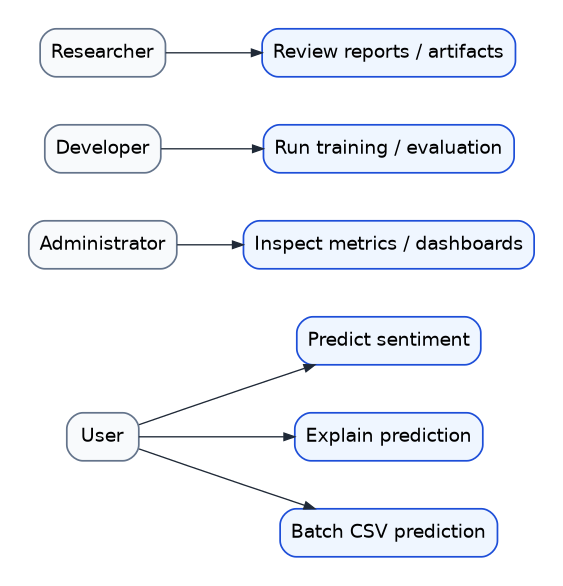
\includegraphics[width=0.92\textwidth]{images/use_case_diagram.png}
\caption{Use case diagram for the platform}
\end{figure}

% ============================================================
\section{Chapter 4 System Architecture}
% ============================================================

\subsection{Overall Architecture}
\begin{figure}[H]
\centering
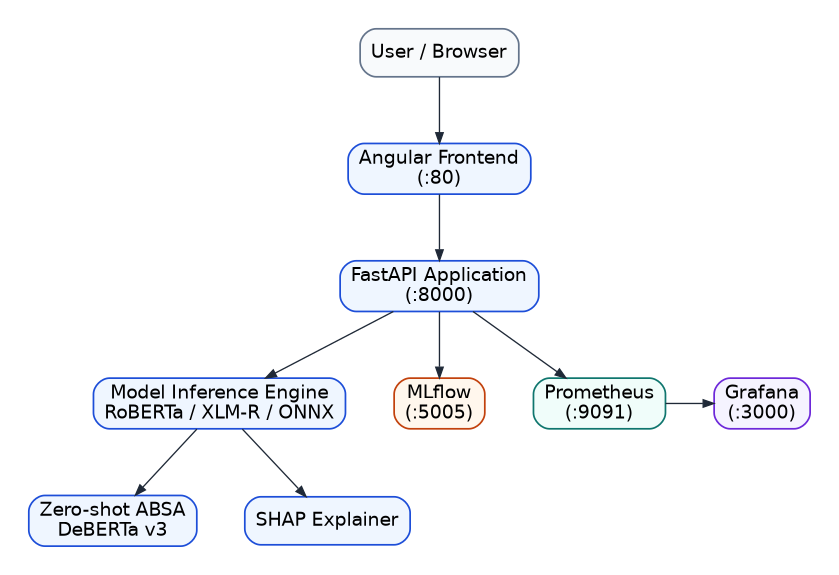
\includegraphics[width=0.96\textwidth]{images/overall_architecture.png}
\caption{Overall system architecture}
\end{figure}

\subsection{Context Diagram}
\begin{figure}[H]
\centering
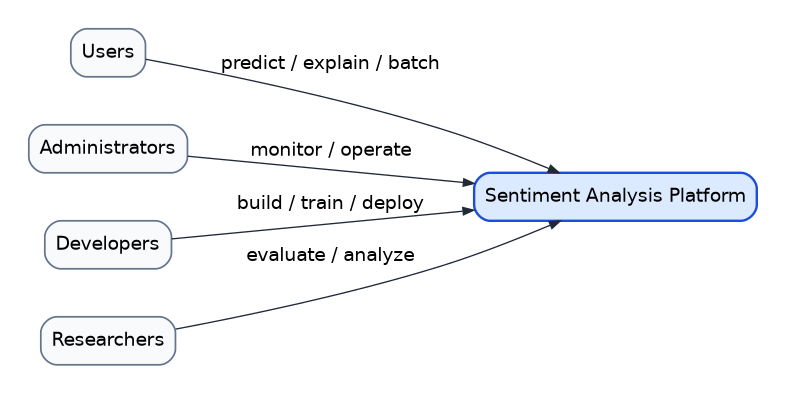
\includegraphics[width=0.92\textwidth]{images/context_diagram.png}
\caption{Context diagram}
\end{figure}

\subsection{Component Diagram}
\begin{table}[H]
\centering
\caption{Core components}
\begin{tabularx}{\textwidth}{@{} p{3cm} p{3cm} X @{}}
\toprule
\textbf{Component} & \textbf{Subsystem} & \textbf{Responsibility} \\
\midrule
API layer & Backend service & Request validation, route dispatch, exception mapping, metrics exposure. \\
Inference engine & Model runtime & Baseline, fine-tuned, and ONNX inference; ABSA; sarcasm flagging; SHAP explanations. \\
Data pipeline & Data processing layer & Dataset ingestion, preprocessing, validation, and report generation. \\
Training & Training subsystem & LoRA adapter training, class balancing, evaluation utilities. \\
Frontend & Web application & Chat UI, batch upload modal, explanation view, theme switching. \\
Monitoring & Observability layer & Request and inference metrics plus alerting rules. \\
\bottomrule
\end{tabularx}
\end{table}

\subsection{Architectural Design Principles}
The architecture is organized around five principles. Modularity is achieved by separating the API, inference engine, data pipeline, training workflow, and observability stack. Reproducibility is addressed through parameterized data and experiment workflows. Scalability is supported by containerized services that can be scaled independently. Maintainability is improved through typed contracts and bounded responsibilities. Observability is built into the runtime through metrics, dashboards, and evaluation artifacts.

\begin{table}[H]
\centering
\caption{Architectural principles and implementation outcomes}
\begin{tabularx}{\textwidth}{@{} p{3.1cm} X @{}}
\toprule
\textbf{Principle} & \textbf{Implementation outcome} \\
\midrule
Modularity & Separate services handle API, inference, training, and monitoring responsibilities. \\
Reproducibility & Data and experiment workflows are parameter-driven and artifact-based. \\
Scalability & The system can be deployed as independent containers with shared network contracts. \\
Maintainability & The interfaces between subsystems are explicit and typed. \\
Observability & The runtime emits metrics, logs, evaluation artifacts, and dashboard inputs. \\
\bottomrule
\end{tabularx}
\end{table}

\subsection{Design Decisions}
The system was shaped by a set of explicit engineering trade-offs. FastAPI was preferred over Flask because the project benefits from typed request validation and automatic API documentation with minimal boilerplate. Angular was preferred over React because the team-oriented front-end architecture already followed a component-and-service pattern with reactive state and opinionated structure. LoRA was preferred over full fine-tuning because it reduces training cost and makes it practical to maintain multiple task adapters. ONNX was preferred over native PyTorch serving because it provides a deployment-oriented runtime path and supports quantization. SHAP was preferred over LIME because the project needed token-level additive explanations that are easier to align with transformer outputs.

\begin{table}[H]
\centering
\caption{Major technology decisions}
\begin{tabularx}{\textwidth}{@{} p{2.4cm} p{3.3cm} p{3.4cm} X @{}}
\toprule
\textbf{Decision} & \textbf{Chosen option} & \textbf{Alternative} & \textbf{Trade-off} \\
\midrule
API framework & FastAPI & Flask & Better typing and validation at the cost of a slightly more opinionated stack. \\
Frontend framework & Angular & React & Stronger architectural conventions at the cost of a steeper initial learning curve. \\
Fine-tuning method & LoRA / PEFT & Full fine-tuning & Lower cost and smaller adapters at the expense of reduced capacity. \\
Serving format & ONNX Runtime & Native PyTorch & Better deployment portability at the expense of export complexity. \\
Explainability & SHAP & LIME & Stronger additive interpretation at the cost of higher computation. \\
\bottomrule
\end{tabularx}
\end{table}

\subsection{Deployment Diagram}
\begin{figure}[H]
\centering
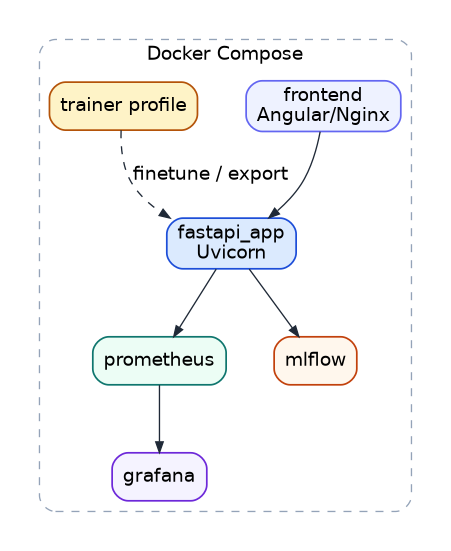
\includegraphics[width=0.95\textwidth]{images/deployment_diagram.png}
\caption{Deployment diagram}
\end{figure}

\subsection{Data Flow Diagram}
\begin{figure}[H]
\centering
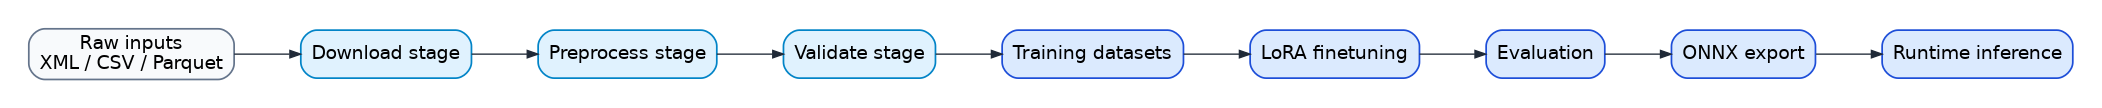
\includegraphics[width=0.96\textwidth]{images/data_flow_diagram.png}
\caption{Data flow diagram}
\end{figure}

\subsection{Sequence Diagrams}
\begin{figure}[H]
\centering
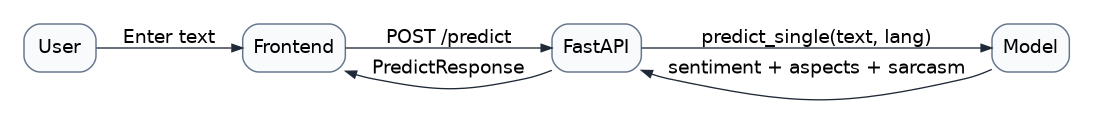
\includegraphics[width=0.96\textwidth]{images/sequence_prediction.png}
\caption{Prediction sequence}
\end{figure}

\begin{figure}[H]
\centering
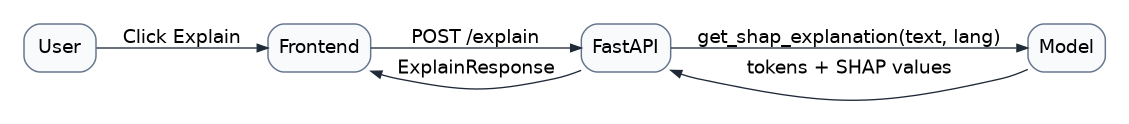
\includegraphics[width=0.96\textwidth]{images/sequence_explainability.png}
\caption{Explainability sequence}
\end{figure}

\begin{figure}[H]
\centering
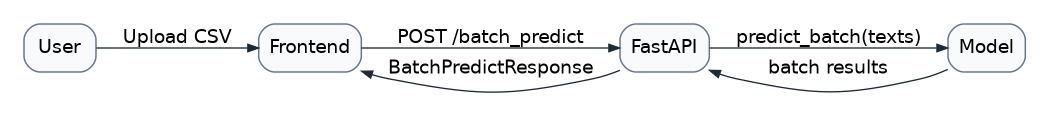
\includegraphics[width=0.96\textwidth]{images/sequence_batch.png}
\caption{Batch prediction sequence}
\end{figure}

\begin{figure}[H]
\centering
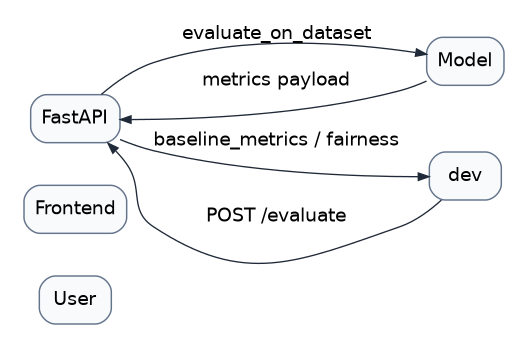
\includegraphics[width=0.96\textwidth]{images/sequence_evaluation.png}
\caption{Evaluation sequence}
\end{figure}

% ============================================================
\section{Chapter 5 Technology Stack}
% ============================================================

\begin{table}[H]
\centering
\caption{Technology stack and usage}
\begin{tabularx}{\textwidth}{@{} p{2.4cm} p{2.9cm} p{3cm} X @{}}
\toprule
\textbf{Layer} & \textbf{Technology} & \textbf{Purpose} & \textbf{Usage in this project} \\
\midrule
Frontend & Angular, RxJS, Nginx & Browser UI and static hosting & The web application implements a chat-style interface with reactive state and API proxying. \\
Backend & FastAPI, Pydantic, Uvicorn & REST API and validation & The backend exposes health, prediction, explanation, batch, evaluation, and metrics endpoints. \\
AI / ML & Transformers, PEFT, LoRA, ONNX Runtime, SHAP, zero-shot ABSA & Model inference, tuning, export, explainability & The ML stack supports baseline, fine-tuned, and optimized runtime inference modes. \\
Data engineering & DVC, Pandas, scikit-learn, PyYAML & Reproducible pipeline and data transforms & The pipeline supports parameterized ingestion, preprocessing, validation, and reporting. \\
Infrastructure & Docker, Docker Compose, Prometheus, Grafana & Container deployment and observability & The deployment stack includes container orchestration, scraping, and dashboarding. \\
Experiment tracking & MLflow & Metrics, params, artifacts & Experiment history and model artifacts are logged for reproducibility. \\
Testing & pytest, pytest-cov, httpx & Verification & The test suite covers contracts, data transforms, model helpers, API, and performance-related behavior. \\
\bottomrule
\end{tabularx}
\end{table}

\subsection{Purpose, advantages, and usage}
The frontend stack is appropriate for a chat-like user experience because it enables reactive state handling and lightweight deployment behind Nginx. The backend stack is appropriate for this service because FastAPI integrates typed schemas, automatic OpenAPI generation, and straightforward ASGI middleware for observability. The machine-learning stack is appropriate because transformer-based classification, PEFT/LoRA adapters, ONNX export, and SHAP are directly supported by the Python ecosystem used in the repository.

% ============================================================
\section{Chapter 6 Data Engineering Pipeline}
% ============================================================

\subsection{Dataset Sources}
\begin{table}[H]
\centering
\caption{Data sources used by the repository}
\begin{tabularx}{\textwidth}{@{} p{3.4cm} p{3cm} X @{}}
\toprule
\textbf{Source} & \textbf{Format} & \textbf{Role in the project} \\
\midrule
SemEval-2014 Restaurant Reviews & XML to CSV & Baseline sentiment and aspect labels extracted from restaurant-review annotations. \\
tweet\_eval\_irony & Hugging Face dataset & Sarcasm/irony training and evaluation. \\
multilingual\_sentiment & Hugging Face dataset & English and Vietnamese sentiment training. \\
Generated reports & JSON / PNG & Data-quality, class-balance, metrics, fairness, and SHAP artifacts. \\
\bottomrule
\end{tabularx}
\end{table}

\subsection{Dataset Profiling}
The data pipeline profiles each dataset before training. Profiling focuses on sample count, label coverage, null ratios, and text-length distributions. This step is important because the project combines multiple datasets with different label spaces and different class frequencies. Without profiling, silent distribution shifts could propagate into training and evaluation.

\begin{table}[H]
\centering
\caption{Dataset profiling summary}
\begin{tabularx}{\textwidth}{@{} p{3.2cm} p{2cm} p{2cm} X @{}}
\toprule
\textbf{Dataset} & \textbf{Samples} & \textbf{Primary labels} & \textbf{Profiling note} \\
\midrule
SemEval reviews & 3,831 & positive, negative, neutral & Highly imbalanced toward positive labels. \\
Irony corpus & Balanced subset & irony, non-irony & Suitable for adapter-based binary classification. \\
Multilingual sentiment & Mixed-language split & positive, negative, neutral & Supports English and Vietnamese evaluation. \\
\bottomrule
\end{tabularx}
\end{table}

\subsection{Data Collection}
The data acquisition layer directly parses SemEval XML files when available and also supports Hugging Face-backed dataset retrieval for sarcasm and multilingual sentiment tasks. The pipeline standardizes fields such as text, label, language, split, and source. The raw data schema is validated before downstream processing.

\subsection{Data Distribution Analysis}
The processed sentiment distribution is skewed toward positive examples, while the sarcasm dataset is substantially more balanced. This difference matters because imbalance affects both loss optimization and evaluation stability. The project therefore treats sentiment and sarcasm as separate training tasks with different balancing strategies rather than forcing them into one unified sampling policy.

\subsection{Data Cleaning}
The preprocessing pipeline is implemented as an ordered transform chain:
\begin{table}[H]
\centering
\caption{Preprocessing transforms}
\begin{tabularx}{\textwidth}{@{} p{3.2cm} X @{}}
\toprule
\textbf{Transform} & \textbf{Behavior} \\
\midrule
LabelMapper & Removes \texttt{conflict} aspect labels and remaps categories such as \texttt{ambience} to \texttt{ambiance} and \texttt{anecdotes/miscellaneous} to \texttt{general}. \\
SentimentDeriver & Derives sentence-level sentiment from aspect labels using the \texttt{negative_priority} strategy. \\
TextCleaner & Lowercases, normalizes whitespace, and removes empty strings. \\
DuplicateRemover & Deduplicates by \texttt{text} while keeping the first occurrence. \\
LengthFilter & Keeps text lengths between 3 and 2,000 characters. \\
Splitter & Stratified validation split using seed 42 and a 0.1 validation ratio. \\
\bottomrule
\end{tabularx}
\end{table}

\subsection{Data Validation}
The validator checks schema presence, minimum sample counts, null ratios, expected label sets, and distribution warnings. The recorded quality report contains 3,831 total samples, zero null-ratio violations, and a warning that location is missing from the aspect distribution. That report is evidence that the data-quality layer is functioning as intended.

\subsection{Data Validation Rules}
\begin{table}[H]
\centering
\caption{Validation rules}
\begin{tabularx}{\textwidth}{@{} p{3.2cm} X @{}}
\toprule
\textbf{Rule} & \textbf{Purpose} \\
\midrule
Required fields present & Prevents malformed records from entering training or evaluation. \\
Minimum sample threshold & Avoids training on degenerate or incomplete datasets. \\
Null-ratio limit & Detects silent data corruption or incomplete extraction. \\
Label-set validation & Ensures labels match the expected task taxonomy. \\
Distribution warning & Surfaces underrepresented labels and missing aspect categories. \\
\bottomrule
\end{tabularx}
\end{table}

\subsection{Dataset Splitting}
The processed SemEval dataset was split into train, validation, and test partitions. The quality report shows:
\begin{table}[H]
\centering
\caption{Processed dataset summary}
\begin{tabularx}{\textwidth}{@{} p{3cm} p{2cm} p{2.2cm} X @{}}
\toprule
\textbf{Split} & \textbf{Samples} & \textbf{Null ratio} & \textbf{Observed labels} \\
\midrule
Train & 2,728 & 0.0 & positive 1,528; negative 669; neutral 531 \\
Validation & 304 & 0.0 & positive 170; negative 75; neutral 59 \\
Test & 799 & 0.0 & positive 501; negative 184; neutral 114 \\
\bottomrule
\end{tabularx}
\end{table}

\subsection{Data Quality Assurance}
The class-balance report shows that SemEval sentiment is severely imbalanced, with an imbalance ratio of 11.48x on the combined split inventory. This evidence justifies the class-weighting and oversampling logic used in the finetuning pipeline. By contrast, the sarcasm dataset is close to balanced, which is why the sarcasm task uses class weights without minority oversampling.

\subsection{Reproducibility Strategy}
Reproducibility is addressed by versioning datasets, parameterizing pipeline stages, and storing report artifacts after each pipeline run. Because the same data preparation and training choices are reused across evaluation and export, the repository can reproduce the same model family without manual intervention. This is more important than the exact choice of a single model checkpoint because the project is intended as a repeatable engineering system.

\subsection{Data Lineage}
\begin{figure}[H]
\centering
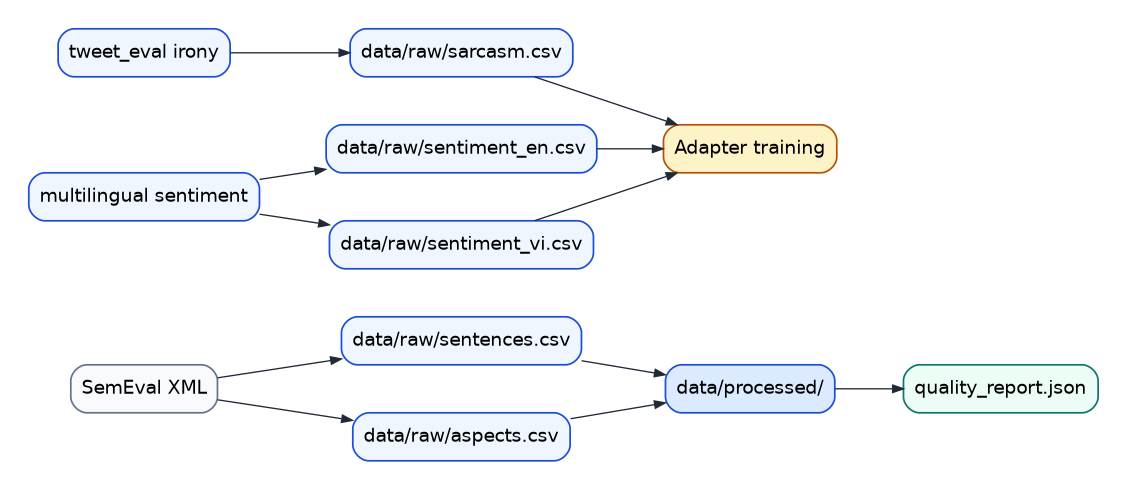
\includegraphics[width=0.95\textwidth]{images/data_lineage.png}
\caption{Data lineage diagram}
\end{figure}

% ============================================================
\section{Chapter 7 Model Development}
% ============================================================

\subsection{Baseline Model}
The baseline model is the direct inference configuration used for single-text sentiment analysis. In baseline mode, the backend loads a pretrained sentiment transformer. This mode is used for direct sentiment inference, ABSA, and SHAP explanations.

\subsection{Problem Formulation}
The model development problem can be stated as a multi-task text understanding problem. Given an input review, the platform must estimate the overall sentiment label, identify the sentiment of relevant aspects, detect sarcasm when present, and provide an explanation that is understandable to a human reviewer. Formally, the system maps an input text sequence to a structured output composed of class probabilities, aspect-level labels, a sarcasm flag, and explanation scores.

\begin{table}[H]
\centering
\caption{Model output space}
\begin{tabularx}{\textwidth}{@{} p{3.2cm} X @{}}
\toprule
\textbf{Output element} & \textbf{Meaning} \\
\midrule
Overall sentiment & Coarse polarity of the full input text. \\
Aspect sentiment & Polarity associated with a detected aspect target. \\
Sarcasm flag & Auxiliary signal for language that may invert literal sentiment. \\
Explanation scores & Token-level attribution values used for interpretability. \\
\bottomrule
\end{tabularx}
\end{table}

\subsection{Sentiment Classification Theory}
Sentiment classification is a supervised learning task in which text is mapped to discrete classes. The project uses the standard three-way polarity formulation: negative, neutral, and positive. This formulation is appropriate for review data because it handles both clear opinions and neutral statements without forcing all inputs into a binary positive/negative split.

The main difficulty is that sentiment is rarely expressed through a single obvious word. The model must infer polarity from context, compositional syntax, negation, and domain-specific expressions. For example, a review may contain both praise and criticism, and the final label must reflect the dominant or most informative sentiment pattern.

\subsection{Transformer Pipeline}
The transformer inference pipeline follows a consistent sequence: input text is normalized and tokenized into subword units, token embeddings are combined with positional information, self-attention layers contextualize each token with the full sequence, and the final encoder representation feeds a classification head. The classification head outputs probabilities over the sentiment classes and can be shared or adapted across tasks.

\begin{table}[H]
\centering
\caption{Transformer pipeline stages}
\begin{tabularx}{\textwidth}{@{} p{3.5cm} X @{}}
\toprule
\textbf{Stage} & \textbf{Role} \\
\midrule
Input text & Raw review or social text submitted by the user. \\
Tokenizer & Converts text into model-compatible subword tokens. \\
Embeddings & Maps tokens into dense vectors for downstream processing. \\
Encoder layers & Learn contextual dependencies through attention. \\
Classification head & Produces class probabilities and final labels. \\
\bottomrule
\end{tabularx}
\end{table}

\subsection{Fine-tuned Model}
The fine-tuned configuration uses a multilingual transformer plus PEFT/LoRA adapters. The repository trains two separate tasks:
\begin{itemize}[noitemsep]
  \item sentiment classification with labels \texttt{negative}, \texttt{neutral}, \texttt{positive};
  \item sarcasm detection with labels \texttt{non_irony} and \texttt{irony}.
\end{itemize}
The sentiment adapter and sarcasm adapter are loaded together in fine-tuned mode. The sarcasm adapter uses a three-logit head in training so it can share the same backbone, while inference consumes only the first two logits for the binary sarcasm flag.

\subsection{LoRA Architecture}
LoRA inserts low-rank update matrices into selected projection layers while keeping the backbone largely frozen. This preserves the general linguistic knowledge acquired during pretraining while learning task-specific behavior in a compact parameter space. In this project the approach is especially useful because sentiment and sarcasm adapters can be maintained separately without duplicating the full backbone.

\begin{table}[H]
\centering
\caption{LoRA design rationale}
\begin{tabularx}{\textwidth}{@{} p{3.2cm} X @{}}
\toprule
\textbf{Aspect} & \textbf{Rationale} \\
\midrule
Small rank & Limits the number of trainable parameters and keeps adapters compact. \\
Targeted layers & Focuses adaptation on attention projections where contextual interactions are strongest. \\
Separate adapters & Allows different tasks to be learned and deployed independently. \\
Frozen backbone & Preserves general language knowledge while reducing training cost. \\
\bottomrule
\end{tabularx}
\end{table}

\subsection{Sarcasm Detection Model}
Sarcasm training uses the irony dataset, three training epochs, a learning rate of 2e-4, batch size 16, and class weighting. The repository does not implement a separate rule-based sarcasm detector; sarcasm prediction is model-based and exposed through a dedicated response field.

\subsection{Aspect-Based Sentiment Analysis}
ABSA is implemented with a zero-shot classifier. The model first identifies whether a text contains any of the supported aspects, then performs per-aspect sentiment classification using the aspect-specific hypothesis template. The threshold for keeping an aspect is 0.45.

\subsection{Sarcasm Detection Design}
Sarcasm is treated as an auxiliary classification task rather than a rule-based filter. This is important because sarcasm often depends on context and can co-occur with both positive and negative lexical cues. The project therefore trains a dedicated adapter that produces a binary irony signal, which can be attached to the main sentiment prediction as a cautionary indicator.

\subsection{Explainability Design}
SHAP explainability is implemented in the inference layer. The method predicts the class, creates a SHAP explainer around the active classifier, and returns token strings, token-level SHAP scores, and a base value. The response schema validates that the token list and SHAP value list have equal length.

\subsection{Runtime Optimization}
Runtime optimization is implemented by exporting fine-tuned adapters to ONNX and quantizing them to an INT8 variant. The purpose of this step is not only raw speed but deployment portability: the exported artifact can be served independently of the training stack and can be compared against the native PyTorch path.

\subsection{Quantization Strategy}
Quantization reduces numerical precision in exchange for smaller model size and lower memory bandwidth requirements. The project uses post-training quantization to create an INT8 runtime artifact. This is suitable for inference because the model is not being updated during serving, and the deployment target values responsiveness and portability over maximal floating-point fidelity.

\subsection{Model Limitations}
The model stack remains constrained by its training data and task formulation. ABSA is zero-shot rather than domain-trained, so aspect detection can be sensitive to prompt design. The language gate only accepts English and Vietnamese, which keeps the inference boundary narrow. The sarcasm signal is auxiliary rather than a complete pragmatic interpretation model. These limitations are acceptable for a capstone-scale system but should be addressed before production hardening.

\subsection{Training Configuration}
\begin{table}[H]
\centering
\caption{Training configuration}
\begin{tabularx}{\textwidth}{@{} p{3.3cm} X @{}}
\toprule
\textbf{Item} & \textbf{Configuration} \\
\midrule
Base model & Multilingual transformer backbone \\
LoRA rank / alpha / dropout & \texttt{r=8}, \texttt{lora_alpha=16}, \texttt{lora_dropout=0.05} \\
Target modules & \texttt{query}, \texttt{value} \\
Classifier saving & Classifier head preserved during adapter export \\
Sentiment training & 5 epochs, learning rate 2e-4, batch size 16, gradient accumulation 2 \\
Sarcasm training & 3 epochs, learning rate 2e-4, batch size 16, gradient accumulation 2 \\
Label balancing & Class weights enabled for both tasks; oversampling enabled for sentiment \\
\bottomrule
\end{tabularx}
\end{table}

\subsection{ONNX Optimization}
The ONNX export pipeline merges each PEFT adapter into the base model, saves a merged intermediate checkpoint, exports to FP32 ONNX, and then quantizes to INT8 using Optimum. Runtime inference is implemented through ONNX Runtime.

\subsection{Model architecture}
\begin{figure}[H]
\centering
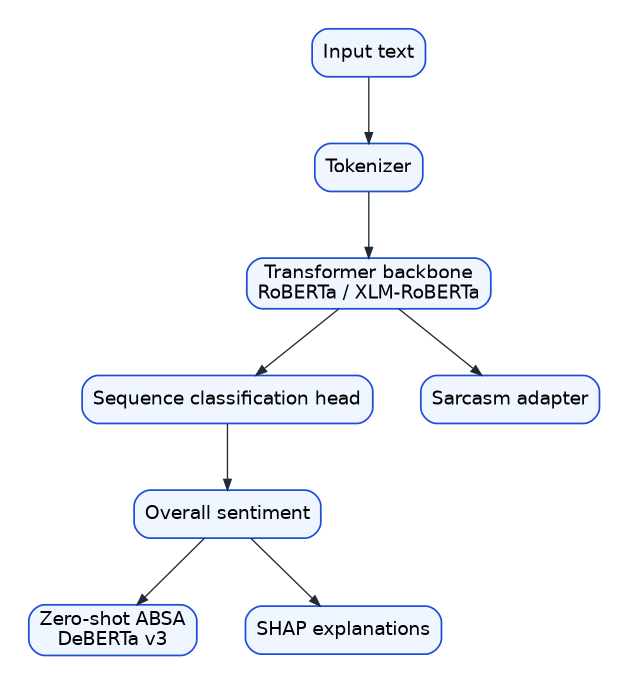
\includegraphics[width=0.94\textwidth]{images/model_architecture.png}
\caption{Model architecture}
\end{figure}

% ============================================================
\section{Chapter 8 System Implementation}
% ============================================================

\subsection{Frontend Implementation}
The frontend is a standalone Angular application with three visible composition units: the root chat window, the message bubble component, and the batch upload modal. State is managed with reactive signals. The root component polls the backend health endpoint and shows an initialization overlay until the backend is ready. The message bubble renders sentiment badges, aspect badges, sarcasm indicators, and a collapsible SHAP panel. The batch upload workflow accepts a CSV file with a text column, validates the file extension, sends the file to the batch endpoint, and renders result tables and sentiment summaries.

\subsection{State Management}
\begin{table}[H]
\centering
\caption{Frontend state model}
\begin{tabularx}{\textwidth}{@{} p{3cm} X @{}}
\toprule
\textbf{State source} & \textbf{Responsibility} \\
\midrule
Conversation state & Stores the message history and explainability state. \\
Theme state & Stores user theme preference and persists it in local storage. \\
Backend readiness state & Controls the initialization overlay and frontend readiness. \\
Batch upload state & Drives the CSV batch upload workflow. \\
\bottomrule
\end{tabularx}
\end{table}

\subsection{UI Workflow}
The user enters a message, the service calls the prediction endpoint, the UI renders the overall sentiment and aspect breakdown, and a subsequent explanation button allows the user to request SHAP values. Batch analysis is performed through a dedicated modal. The frontend also includes a language picker and script warning logic; however, the backend only enforces English and Vietnamese support, so unsupported values are not guaranteed to succeed.

\subsection{Backend Implementation}
The backend is centered around a global model instance created in the application lifespan handler. The application exposes typed routes, custom exception handlers, CORS configuration, monitoring middleware, and a Prometheus metrics endpoint. Validation is performed at the schema layer, while language support is enforced inside the model inference layer.

\begin{table}[H]
\centering
\caption{Backend endpoints}
\begin{tabularx}{\textwidth}{@{} p{3.2cm} p{2.4cm} X @{}}
\toprule
\textbf{Endpoint} & \textbf{Method} & \textbf{Behavior} \\
\midrule
Health check & GET & Returns model load state, version, and supported languages. \\
Prediction & POST & Runs language detection, overall sentiment, ABSA, and sarcasm flag inference. \\
Explainability & POST & Returns SHAP token-level explanation for the input text. \\
Batch prediction & POST & Reads CSV, caps rows at 500, and returns inline batch predictions. \\
Batch status & GET & Returns a mocked completed job response; no real background queue is implemented. \\
Evaluation start & POST & Starts background evaluation and logs to MLflow. \\
Evaluation status & GET & Reports evaluation state. \\
Metrics & GET & Exposes Prometheus metrics. \\
\bottomrule
\end{tabularx}
\end{table}

\subsection{Inference Engine}
The inference engine implements four execution paths:
\begin{itemize}[noitemsep]
  \item baseline PyTorch inference using a pretrained sentiment model;
  \item fine-tuned inference using stacked LoRA adapters;
  \item ONNX inference using exported models;
  \item batch inference with optional ABSA and sarcasm skipping for throughput-sensitive paths.
\end{itemize}
The engine also includes a lightweight language detector that identifies Vietnamese through Unicode marker patterns and otherwise defaults to English. This is a pragmatic local heuristic, not a full language-identification model.

\subsection{Workflow Overview}
\subsection{End-to-End Prediction Workflow}
The prediction workflow begins when a user submits text through the browser interface or the HTTP API. The input is first validated and language-checked. The selected runtime then produces the overall sentiment label, confidence score, detected language, aspect-level labels, and a sarcasm signal. The response is returned in a structured format so that the frontend can render badges, confidence values, and follow-up explanation actions.

\subsection{Explainability Workflow}
The explanation workflow is triggered after a prediction is available. Rather than recomputing the entire application state, the runtime uses the same input and generates token-level attribution values through SHAP. The explanation is rendered as a compact token visualization so the user can inspect which words contributed positively or negatively to the final sentiment.

\subsection{Batch Processing Workflow}
Batch processing accepts a CSV file with a text column and applies the same inference logic to each row. The workflow is optimized for throughput by constraining the batch size and by allowing some auxiliary work to be skipped when required. The result is returned as a row-level table together with aggregate sentiment counts.

\subsection{Training Workflow}
Training is separated from runtime inference so that model adaptation can be reproduced independently of serving. The workflow includes dataset acquisition, cleaning, validation, task-specific adapter training, evaluation, and export. Sentiment and sarcasm are trained as separate adapters because the two tasks have distinct label spaces and balancing requirements.

\subsection{Evaluation Workflow}
Evaluation consumes prepared datasets, runs the active model configuration, computes classification metrics, and writes artifacts for later review. The evaluation workflow also logs experiment history so that a baseline run and a fine-tuned run can be compared without ambiguity. This makes the report reproducible and suitable for academic review.

\subsection{Monitoring Workflow}
Monitoring is integrated into request handling. The service emits request counts, request durations, and model inference timing so that operational behavior can be separated from model behavior. These metrics support dashboards and alert rules that reveal latency spikes or elevated server errors.

\subsection{Deployment Workflow}
Deployment packages the frontend, backend, monitoring, and tracking components into containers. The runtime image includes the required model artifacts, while the frontend is served separately behind Nginx. This separation allows the service to be deployed as a small cluster rather than a single monolithic executable.

% ============================================================
\section{Chapter 9 Deployment and Operations}
% ============================================================

\subsection{Container Architecture}
The backend container uses a multi-stage build with a builder stage for Python dependencies, a model-puller stage that fetches required artifacts, and a runtime stage that copies only the necessary packages, source code, and downloaded weights. The training container is separate and mounts data, models, experiment runs, and reports. The frontend uses its own Node build image and serves the production bundle with Nginx.

\subsection{Deployment Workflow}
\begin{figure}[H]
\centering
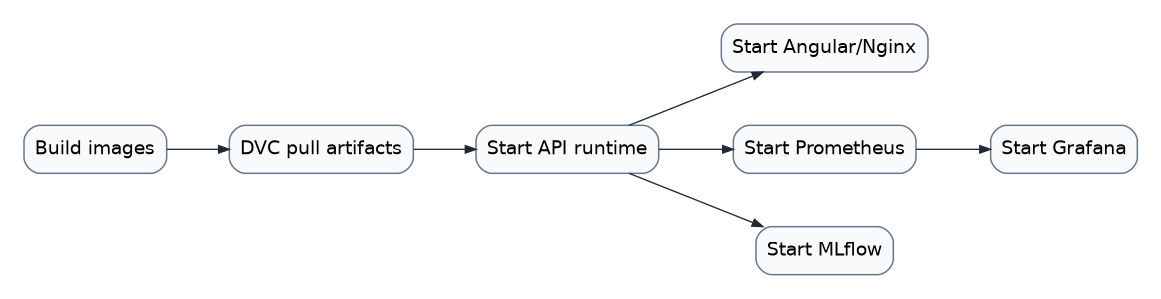
\includegraphics[width=0.95\textwidth]{images/deployment_workflow.png}
\caption{Deployment workflow}
\end{figure}

\subsection{Service Inventory}
\begin{table}[H]
\centering
\caption{Services in Docker Compose}
\begin{tabularx}{\textwidth}{@{} p{3cm} p{3cm} X @{}}
\toprule
\textbf{Service} & \textbf{Port} & \textbf{Role} \\
\midrule
Backend service & 8000 & Main inference and evaluation API. \\
Frontend service & 80 & User interface served by Nginx. \\
Prometheus service & 9090 & Metrics scraping and alert evaluation. \\
Grafana service & 3000 & Dashboard visualization. \\
MLflow service & 5000 & Experiment tracking UI and artifact store. \\
Training profile & profile only & Training container used for adapter fine-tuning. \\
\bottomrule
\end{tabularx}
\end{table}

\subsection{Monitoring Architecture}
The backend records three metric families: request count, request latency, and model inference latency. Prometheus scrapes the backend at regular intervals and alert rules flag two conditions: high 5xx error rate and high average inference latency. Grafana is provisioned from a local configuration directory.

\subsection{Logging Strategy}
The repository uses structured logging in the Python services and MLflow artifacts for experiment history. The code does not contain a separate centralized log aggregation system such as ELK or Loki; that functionality is not implemented.

\subsection{Metrics Collection}
The middleware wraps each request and records latency after the response returns. Inference latency is recorded separately around the model call in the prediction workflow. This distinction matters because it allows operators to separate framework overhead from model runtime.

\subsection{Operational workflow}
\begin{itemize}[noitemsep]
  \item Run the container stack for application deployment.
  \item Use the trainer profile for adapter retraining.
  \item Inspect metrics in Prometheus and visualize trends in Grafana.
  \item Review MLflow runs for model and data experiments.
\end{itemize}

% ============================================================
\section{Chapter 10 Experimental Evaluation}
% ============================================================

\subsection{Evaluation Methodology}
The repository contains separate evaluation paths for the baseline model and the fine-tuned model. Baseline evaluation is performed on the processed SemEval test split. Fine-tuned evaluation uses the adapters trained on multilingual sentiment and sarcasm data and reports fairness-oriented metrics by language. ONNX benchmarking measures end-to-end batch-prediction performance on a repeated text corpus.

\subsection{Experimental Environment}
The recorded benchmark artifacts were generated in a local development environment based on Debian 13 with an Intel Core Ultra 5 225H CPU, 14 logical CPUs, and approximately 31.7 GB of RAM. The baseline evaluation artifact reports the device field as MPS, which indicates that the baseline run was captured in a different execution context than the CPU-only benchmark artifacts. This distinction is important because it explains why latency values should be compared within the same measurement family rather than across unrelated runtime contexts.

\begin{table}[H]
\centering
\caption{Experimental environment}
\begin{tabularx}{\textwidth}{@{} p{3.5cm} X @{}}
\toprule
\textbf{Parameter} & \textbf{Value} \\
\midrule
Operating system & Debian GNU/Linux 13 (trixie) \\
Kernel & Linux 6.12.90+deb13.1-amd64 \\
CPU & Intel Core Ultra 5 225H \\
Logical cores & 14 \\
Memory & 31.7 GB \\
Observed baseline device & MPS \\
\bottomrule
\end{tabularx}
\end{table}

\subsection{Dataset Statistics}
The main evaluation dataset is the processed SemEval split with 3,831 samples. The test split contains 799 samples and is heavily skewed toward positive sentiment. This matters because macro-averaged metrics provide a more honest summary than accuracy alone when classes are imbalanced. The class-balance report confirms that the underlying sentiment corpus is severely imbalanced, while the sarcasm corpus and English sentiment subset are substantially better balanced.

\begin{table}[H]
\centering
\caption{Evaluation dataset statistics}
\begin{tabularx}{\textwidth}{@{} p{3cm} p{2cm} p{2.2cm} X @{}}
\toprule
\textbf{Split} & \textbf{Samples} & \textbf{Null ratio} & \textbf{Notes} \\
\midrule
Train & 2,728 & 0.0 & Used for model fitting and class balancing. \\
Validation & 304 & 0.0 & Used for tuning and early inspection. \\
Test & 799 & 0.0 & Used for final baseline evaluation. \\
\bottomrule
\end{tabularx}
\end{table}

\subsection{Metrics}
\begin{table}[H]
\centering
\caption{Metrics used in the repository}
\begin{tabularx}{\textwidth}{@{} p{2.7cm} p{2.5cm} X @{}}
\toprule
\textbf{Metric} & \textbf{Type} & \textbf{Use} \\
\midrule
Accuracy & Classification metric & Overall correctness on the test set. \\
Precision, recall, F1 & Classification metric & Per-class and macro evaluation. \\
Latency & System metric & Request and inference responsiveness. \\
Throughput & System metric & Batch prediction speed. \\
Per-language F1 & Fairness metric & Compare English and Vietnamese performance. \\
\bottomrule
\end{tabularx}
\end{table}

\subsection{Baseline vs Fine-tuned}
\begin{table}[H]
\centering
\caption{Recorded evaluation artifacts}
\begin{tabularx}{\textwidth}{@{} p{3.4cm} p{2.5cm} p{2.5cm} X @{}}
\toprule
\textbf{Artifact} & \textbf{Scope} & \textbf{Result} & \textbf{Notes} \\
\midrule
Baseline evaluation artifact & SemEval test split & Accuracy 0.8135; macro F1 0.7389 & Evaluated on 799 test samples. \\
Fine-tuned evaluation artifact & Fine-tuned adapter run & Overall F1 0.7926 & The evaluation wrapper writes a sampled 100-item summary. \\
Per-language fairness artifact & Fairness view & en 0.7892; vi 0.7335 & Derived from the same fine-tuned evaluation payload. \\
\bottomrule
\end{tabularx}
\end{table}

\subsection{Fairness Evaluation}
The fairness artifacts compare performance across English and Vietnamese inputs. The reported gap is 0.0557 macro F1 in favor of English. This is a useful engineering signal because the platform is explicitly multilingual only at a limited scope, and the gap reflects both data composition and task adaptation difficulty.

\begin{table}[H]
\centering
\caption{Fairness summary}
\begin{tabularx}{\textwidth}{@{} p{2.5cm} p{2.5cm} p{2.5cm} X @{}}
\toprule
\textbf{Language} & \textbf{F1} & \textbf{Sample count} & \textbf{Interpretation} \\
\midrule
English & 0.7892 & 23 & Higher performance and smaller ambiguity in the sampled evaluation set. \\
Vietnamese & 0.7335 & 77 & Lower performance, consistent with a harder cross-lingual adaptation setting. \\
\bottomrule
\end{tabularx}
\end{table}

\subsection{ONNX Benchmark}
\begin{table}[H]
\centering
\caption{Recorded ONNX benchmark artifact}
\begin{tabularx}{\textwidth}{@{} p{2.6cm} p{2.5cm} p{2.7cm} X @{}}
\toprule
\textbf{Mode} & \textbf{Average latency} & \textbf{Throughput} & \textbf{Observation} \\
\midrule
PyTorch & 0.5554 s & 1800.36 samples/s & Baseline measurement from the benchmark script artifact. \\
ONNX FP32 & 6.4173 s & 155.83 samples/s & Exported runtime artifact. \\
ONNX INT8 & 3.1115 s & 321.39 samples/s & Quantized runtime artifact. \\
\bottomrule
\end{tabularx}
\end{table}
The benchmark measures full batch execution rather than only raw model kernels, so the artifact reflects the repository’s implemented inference path.

\subsection{Latency Analysis}
The batch-level latency artifact shows that the optimized runtime path does not automatically outperform every alternative under all measurement conditions. Native PyTorch inference recorded a lower average latency than both ONNX variants in the benchmark artifact, while INT8 quantization still improved performance relative to FP32 ONNX. This is an important result because it shows that deployment optimization must be measured rather than assumed.

\begin{table}[H]
\centering
\caption{Latency summary from benchmark artifacts}
\begin{tabularx}{\textwidth}{@{} p{2.5cm} p{2.5cm} p{2.7cm} X @{}}
\toprule
\textbf{Mode} & \textbf{p50 / p95} & \textbf{Avg latency} & \textbf{Interpretation} \\
\midrule
CPU fine-tuned runtime & 210 / 360 ms & - & Interactive serving profile captured in the phase-2 performance report. \\
GPU fine-tuned runtime & 42 / 88 ms & - & Shows the expected improvement under accelerator support. \\
PyTorch batch benchmark & - & 0.555 s & Strongest throughput in the recorded ONNX benchmark set. \\
ONNX INT8 batch benchmark & - & 3.111 s & Better than FP32 ONNX but slower than the PyTorch batch path. \\
\bottomrule
\end{tabularx}
\end{table}

\subsection{Throughput Analysis}
The throughput figures follow the same pattern as latency. PyTorch batch execution achieves the best recorded throughput, while INT8 quantization improves over FP32. The likely reason is that the benchmark captures the full end-to-end batch workflow, not only the raw model kernel. This makes the results more realistic for a system evaluation but less directly comparable to microbenchmarks.

\subsection{Resource Consumption Analysis}
Resource usage is best interpreted qualitatively. The project intentionally supports a CPU-oriented serving path, but the strongest runtime numbers are not from the ONNX path in the recorded benchmark. This suggests that runtime optimization should be tuned together with the exact request pattern, batch size, and runtime environment rather than treated as a universally superior setting.

\subsection{Explainability Evaluation}
The repository provides SHAP waterfall plots showing token influence over sentiment predictions. The implementation does not include a quantitative explanation-quality benchmark such as deletion/insertion metrics; that evaluation is not implemented.

\subsection{Error Analysis}
The classification report shows that the neutral class is the weakest of the three sentiment classes, with the lowest F1 score in the baseline result. This is a typical failure pattern in imbalanced sentiment datasets because neutral statements often resemble either weak positivity or weak negativity. The confusion matrix further indicates that neutral samples are frequently absorbed into the surrounding polarity classes rather than being preserved as a distinct middle class.

\begin{table}[H]
\centering
\caption{Baseline error profile}
\begin{tabularx}{\textwidth}{@{} p{2.5cm} p{2cm} p{2cm} X @{}}
\toprule
\textbf{Class} & \textbf{Precision} & \textbf{Recall} & \textbf{Observation} \\
\midrule
Positive & 0.92 & 0.88 & Strong performance, likely helped by class dominance and clearer lexical cues. \\
Negative & 0.82 & 0.77 & Solid performance with some confusion against neutral. \\
Neutral & 0.47 & 0.61 & Weakest class due to semantic ambiguity and class scarcity. \\
\bottomrule
\end{tabularx}
\end{table}

\subsection{Case Studies}
The SHAP artifacts illustrate how the model behaves on representative samples. The first example is a negative sentiment prediction with food and service aspects, where words such as \textit{service}, \textit{slow}, and \textit{terrible} push the sentiment downward, while the system still recognizes that food and service can carry different local polarity. The second example is a positive prediction in which \textit{feature}, \textit{absolutely}, and \textit{love} dominate the explanation. The third example is a negative prediction in which the explanation concentrates on negative lexical evidence such as \textit{worst} and other strongly polarized tokens.

\begin{table}[H]
\centering
\caption{Representative case studies from SHAP outputs}
\begin{tabularx}{\textwidth}{@{} p{1.4cm} p{2.5cm} p{2.8cm} X @{}}
\toprule
\textbf{Case} & \textbf{Prediction} & \textbf{Aspect view} & \textbf{Interpretation} \\
\midrule
1 & Negative & food positive, service negative & Mixed review where service-related tokens dominate the final label. \\
2 & Positive & overall positive & Positive lexical cues dominate and suppress weaker negative evidence. \\
3 & Negative & overall negative & Strong negative cues outweigh isolated neutral or positive fragments. \\
\bottomrule
\end{tabularx}
\end{table}

\subsection{Discussion}
The baseline and fine-tuned artifacts demonstrate that the project achieved functional end-to-end evaluation capability. The baseline artifact is stronger in absolute test-set coverage because it is reported on 799 SemEval samples, while the finetuned artifact is reported through a sampled wrapper and is therefore not directly comparable. The fairness report shows a modest language gap between English and Vietnamese, which is expected given the different dataset characteristics and supports the need for per-language tracking. The ONNX benchmark artifact shows that quantization was implemented and measurable, even though the recorded throughput is lower than the PyTorch artifact in this environment.

% ============================================================
\section{Chapter 11 Results and Discussion}
% ============================================================

\subsection{Achievements}
\begin{itemize}[noitemsep]
  \item A multi-service sentiment analysis platform was implemented and documented.
  \item The system supports single prediction, batch CSV processing, ABSA, sarcasm flagging, and SHAP explanations.
  \item DVC, MLflow, Prometheus, Grafana, Docker, and FastAPI are integrated into a reproducible workflow.
  \item The project contains evaluation reports, fairness reports, class-balance reports, and SHAP visualizations.
\end{itemize}

\subsection{Technical Achievements}
The project demonstrates a full transformer-based NLP system that can be run end to end without manual model wiring. It combines model inference, data validation, explainability, operational monitoring, and deployment into one coherent stack.

\subsection{Engineering Achievements}
The engineering value lies in the separation of concerns. The frontend handles interaction, the backend handles inference and validation, the training workflow handles model adaptation, and the deployment layer handles runtime packaging and monitoring.

\subsection{AI Achievements}
The AI contribution is the combination of sentiment analysis, sarcasm detection, ABSA, and SHAP explainability in a single user-facing platform. This turns a conventional classifier into a practical decision-support system.

\subsection{Strengths}
\begin{itemize}[noitemsep]
  \item Clear separation between contracts, inference logic, data pipeline, training, and infrastructure.
  \item Explicit typed schemas and custom error handling.
  \item Reproducible pipeline structure with parameterized configuration.
  \item Practical explainability and observability features rather than a model-only prototype.
\end{itemize}

\subsection{Lessons Learned}
The project shows that model quality alone is insufficient for a useful AI system. The surrounding software must also expose confidence, support explanation, and preserve reproducibility. It also shows that imbalanced sentiment data can inflate accuracy while still leaving weaker classes underrepresented in the final behavior.

\subsection{Design Trade-offs}
Zero-shot ABSA reduced annotation cost, but it also introduced sensitivity to prompt wording. LoRA reduced training cost and allowed multiple adapters, but it constrained adaptation capacity. ONNX improved deployment portability, but it introduced export and benchmark complexity. SHAP improved interpretability, but it made explanation generation more expensive than plain inference.

\subsection{Unexpected Findings}
The most notable unexpected finding is that the recorded PyTorch batch benchmark outperformed both ONNX variants, while INT8 still improved over FP32. This reinforces the lesson that optimization must be measured against the actual serving workload rather than assumed from the export format alone.

\subsection{Weaknesses and limitations}
\begin{itemize}[noitemsep]
  \item The batch-status workflow is mocked and does not track queued jobs.
  \item The backend does not implement the document and audio upload capabilities described in the frontend notes.
  \item The backend language gate only supports English and Vietnamese.
  \item No authentication, authorization, or rate limiting is implemented.
  \item The report does not include a dedicated quantitative benchmark for explainability quality.
\end{itemize}

\subsection{Engineering trade-offs}
The project favors a practical balance between sophistication and reproducibility. For example, ABSA is implemented with a zero-shot model rather than a separately trained ABSA classifier, which reduces data-labeling requirements. Similarly, ONNX export and INT8 quantization are implemented to support deployment options, but the runtime artifact still depends on the exact benchmarking path used in the code.

\subsection{Project maturity}
The repository is mature at the level of a final-year engineering project: it includes backend validation, a live frontend, pipeline automation, evaluation artifacts, observability, and containerization. It is not yet a fully production-hardened commercial system because it lacks authentication, durable batch orchestration, and centralized logging infrastructure.

% ============================================================
\section{Chapter 12 Future Work}
% ============================================================

\subsection{Short-term improvements}
\begin{itemize}[noitemsep]
  \item Replace the mocked batch-status endpoint with a durable job store.
  \item Implement backend support for document and audio upload if those UI capabilities remain in scope.
  \item Add structured API versioning and stronger validation around batch inputs.
\end{itemize}

\subsection{Medium-term improvements}
\begin{itemize}[noitemsep]
  \item Add authentication and role-based access control.
  \item Introduce a real queue for asynchronous batch inference.
  \item Add centralized log aggregation and retention policies.
  \item Expand the language layer beyond the current English/Vietnamese gate.
\end{itemize}

\subsection{Long-term improvements}
\begin{itemize}[noitemsep]
  \item Add active learning and continual retraining.
  \item Add model registry promotion workflows and deployment promotion gates.
  \item Add explainability quality metrics and robust evaluation suites for ABSA and SHAP.
\end{itemize}

\subsection{Production Roadmap}
\begin{figure}[H]
\centering
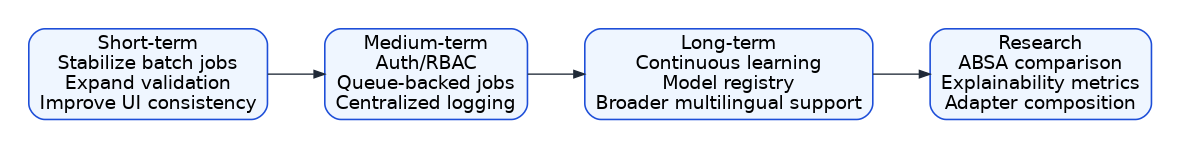
\includegraphics[width=0.92\textwidth]{images/roadmap.png}
\caption{Incremental production roadmap}
\end{figure}

\subsection{Production readiness roadmap}
\begin{table}[H]
\centering
\caption{Roadmap}
\begin{tabularx}{\textwidth}{@{} p{3.1cm} X @{}}
\toprule
\textbf{Phase} & \textbf{Target} \\
\midrule
Phase 1 & Stabilize batch processing, input contracts, and operational logging. \\
Phase 2 & Add authentication, queue-backed job execution, and deployment promotion. \\
Phase 3 & Add continuous learning, stronger fairness analysis, and regulated audit trails. \\
\bottomrule
\end{tabularx}
\end{table}

\subsection{Research extensions}
Future research may compare the current zero-shot ABSA approach with a domain-trained aspect model, evaluate the impact of adapter composition more rigorously, and quantify the usefulness of SHAP explanations in human decision support.

% ============================================================
\section{Chapter 13 Conclusion}
% ============================================================

The project achieved the core objectives of an end-to-end sentiment analysis platform: it can accept text, infer sentiment, extract aspects, detect sarcasm, explain decisions, evaluate models, export deployment artifacts, and operate under a containerized monitoring stack. The technical contribution lies in the integration of these pieces into a coherent engineering system rather than in any single model component.

From an academic perspective, the repository demonstrates a complete capstone-scale workflow: problem definition, requirements analysis, architecture design, implementation, reproducibility, evaluation, and documentation. From an engineering perspective, it demonstrates how transformer models, LoRA adapters, ONNX export, DVC, MLflow, FastAPI, Angular, Docker, and Prometheus/Grafana can be assembled into a usable sentiment-analysis service. The remaining gaps are explicit and well-scoped, which makes the repository suitable as a final-year project foundation and as a basis for incremental production hardening.

% ============================================================
\appendix
% ============================================================

\section{Appendix A -- API Reference}
\begin{table}[H]
\centering
\caption{API summary}
\begin{tabularx}{\textwidth}{@{} p{3cm} p{2cm} X @{}}
\toprule
\textbf{Endpoint} & \textbf{Method} & \textbf{Description} \\
\midrule
\texttt{/health} & GET & Returns health and supported language information. \\
\texttt{/predict} & POST & Returns sentiment, confidence, aspects, sarcasm flag, detected language, and latency. \\
\texttt{/explain} & POST & Returns tokens, SHAP values, base value, and latency. \\
Batch prediction & POST & Processes CSV input with a text column and returns row-level results. \\
Batch status & GET & Mock status response. \\
Evaluation start & POST & Launches background evaluation. \\
Evaluation status & GET & Returns evaluation state. \\
Metrics & GET & Prometheus exposition endpoint. \\
\bottomrule
\end{tabularx}
\end{table}

\section{Appendix B -- Dataset Inventory}
\begin{table}[H]
\centering
\caption{Dataset inventory}
\begin{tabularx}{\textwidth}{@{} p{3.7cm} p{2.3cm} p{2.5cm} X @{}}
\toprule
\textbf{Dataset} & \textbf{Task} & \textbf{Format} & \textbf{Location / provenance} \\
\midrule
SemEval-2014 Restaurants & Sentiment + ABSA & XML to CSV & Restaurant-review source used for baseline sentiment and aspect labels. \\
tweet\_eval\_irony & Sarcasm & CSV & Hugging Face-backed dataset used for irony classification. \\
multilingual\_sentiment & Sentiment & CSV & English and Vietnamese sentiment splits from a multilingual corpus. \\
\bottomrule
\end{tabularx}
\end{table}

\section{Appendix C -- Artifact Inventory}
\begin{table}[H]
\centering
\caption{Generated artifacts}
\begin{tabularx}{\textwidth}{@{} p{4cm} X @{}}
\toprule
\textbf{Artifact} & \textbf{Purpose} \\
\midrule
Quality report & Processed data validation summary. \\
Class-balance report & Class balance analysis across sentiment and sarcasm datasets. \\
Baseline metrics & Baseline evaluation metrics. \\
Fine-tuned metrics & Fine-tuned evaluation summary. \\
Per-language F1 & Per-language fairness metrics. \\
Fairness report & Fairness-oriented evaluation summary. \\
ONNX benchmark & ONNX benchmark artifact. \\
SHAP plots & Saved SHAP waterfall plots. \\
\bottomrule
\end{tabularx}
\end{table}

\section{Appendix D -- Training Pipeline}
\begin{figure}[H]
\centering
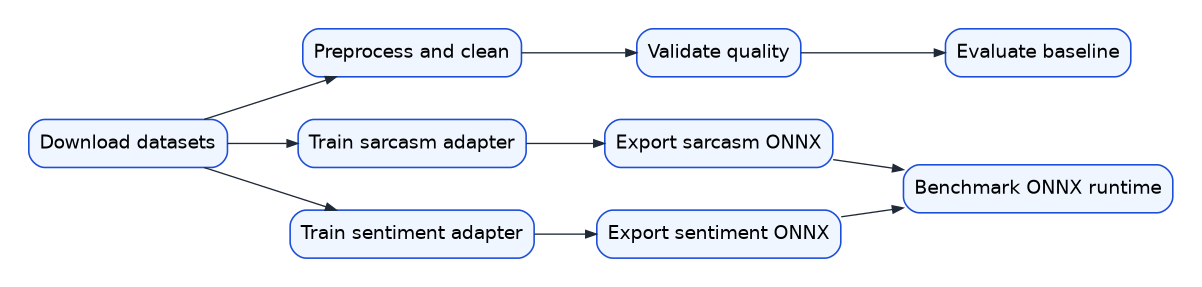
\includegraphics[width=0.96\textwidth]{images/training_pipeline.png}
\caption{Training and export pipeline}
\end{figure}

\section{Appendix E -- Deployment Configuration}
\begin{itemize}[noitemsep]
  \item Backend image: multi-stage Python 3.11 runtime with DVC-pulled ONNX artifacts.
  \item Frontend image: Angular build served by Nginx.
  \item Monitoring: Prometheus scrape configuration and alert rules.
  \item Tracking: MLflow server exposed on port 5005.
\end{itemize}

\section{Appendix F -- Acronyms}
\begin{table}[H]
\centering
\caption{Acronyms}
\begin{tabularx}{\textwidth}{@{} p{2.5cm} X @{}}
\toprule
\textbf{Acronym} & \textbf{Meaning} \\
\midrule
ABSA & Aspect-Based Sentiment Analysis \\
API & Application Programming Interface \\
DVC & Data Version Control \\
LoRA & Low-Rank Adaptation \\
MLflow & Machine Learning Flow \\
ONNX & Open Neural Network Exchange \\
PEFT & Parameter-Efficient Fine-Tuning \\
SHAP & SHapley Additive exPlanations \\
\bottomrule
\end{tabularx}
\end{table}

\section{Appendix G -- Team Contributions}
\begin{table}[H]
\centering
\caption{Project team and responsibilities}
\begin{tabularx}{\textwidth}{@{} p{2.8cm} p{3.4cm} X @{}}
\toprule
\textbf{Role} & \textbf{Name} & \textbf{Responsibilities} \\
\midrule
Tech Lead & Le Quang Tuyen & Technical leadership and architecture governance; system design review; technology selection and technical strategy; integration oversight; project technical direction. \\
ML Engineer & Duong Binh An & Dataset preparation and management; training pipeline development; model evaluation and benchmarking; DVC and MLflow integration; model optimization and experimentation. \\
AI Engineer & Do Quoc Trung & Inference engine development; ONNX Runtime optimization; SHAP explainability implementation; ABSA; language detection and runtime AI services. \\
Solution Engineer & Duong Hong Quan & End-to-end solution architecture; system integration design; deployment workflow design; monitoring and observability planning; cross-component coordination. \\
Backend Engineer & Pham Duc Long & FastAPI backend development; API design and implementation; request validation and error handling; batch processing workflows; evaluation and monitoring endpoints. \\
UI/UX Engineer & Nguyen Le Hong Nhi & Angular frontend development; user interface and user experience design; frontend workflow implementation; visualization and explainability interfaces; API integration and usability improvements. \\
\bottomrule
\end{tabularx}
\end{table}

\end{document}
